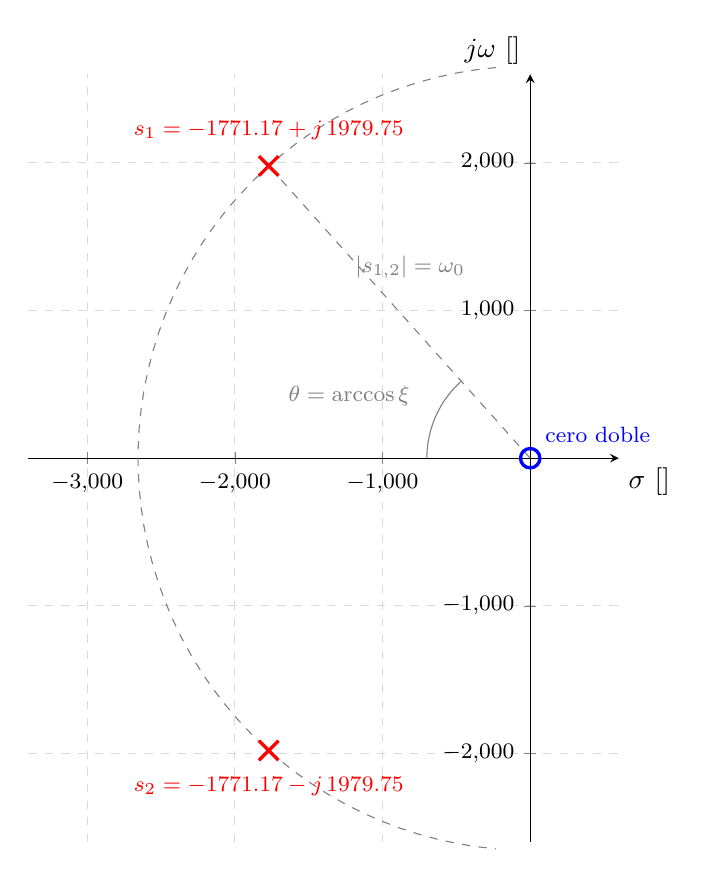
\begin{tikzpicture}
  \begin{axis}[
    % escala igual en ambos ejes: 4000 x 5200 rad/s sobre 7,5 cm x 9,75 cm
    scale only axis, width=7.5cm, height=9.75cm,
    axis lines=middle,
    xlabel={$\sigma$ [\unit{\radian\per\second}]},
    ylabel={$j\omega$ [\unit{\radian\per\second}]},
    xlabel style={at={(ticklabel* cs:1)}, anchor=north west},
    ylabel style={at={(ticklabel* cs:1)}, anchor=south east},
    xmin=-3400, xmax=600, ymin=-2600, ymax=2600,
    xtick={-3000,-2000,-1000},
    ytick={-2000,-1000,1000,2000},
    grid=both, grid style={gray!30, dashed},
    tick label style={font=\footnotesize},
    clip=false,
  ]
    % circunferencia de radio omega_0 sobre la que se ubican los polos
    \addplot[domain=95:265, samples=60, dashed, gray, no marks] ({2656.4*cos(x)}, {2656.4*sin(x)});
    \addplot[dashed, gray, no marks] coordinates {(0,0) (-1771.17,1979.75)};
    \addplot[domain=131.8:180, samples=20, gray, no marks] ({700*cos(x)}, {700*sin(x)});
    \addplot[only marks, mark=x, mark size=5pt, very thick, red]
      coordinates {(-1771.17,1979.75) (-1771.17,-1979.75)};
    \addplot[only marks, mark=o, mark size=3.5pt, very thick, blue] coordinates {(0,0)};
    \node[above=6pt, red, font=\footnotesize] at (axis cs:-1771.17,1979.75)
      {$s_1 = \num{-1771.17} + j\,\num{1979.75}$};
    \node[below=6pt, red, font=\footnotesize] at (axis cs:-1771.17,-1979.75)
      {$s_2 = \num{-1771.17} - j\,\num{1979.75}$};
    \node[above right=2pt, blue, font=\footnotesize] at (axis cs:0,0) {cero doble};
    \node[gray, font=\footnotesize, anchor=south west] at (axis cs:-1250,1150) {$|s_{1,2}| = \omega_0$};
    \node[gray, font=\footnotesize, anchor=east] at (axis cs:-750,420) {$\theta = \arccos\xi$};
  \end{axis}
\end{tikzpicture}
